\documentclass{article}

\usepackage{graphics}

% set font encoding for PDFLaTeX, XeLaTeX, or LuaTeX
\usepackage{ifxetex,ifluatex}
\if\ifxetex T\else\ifluatex T\else F\fi\fi T%
  \usepackage{fontspec}
\else
  \usepackage[T1]{fontenc}
  \usepackage[utf8]{inputenc}
  \usepackage{lmodern}
\fi

\usepackage{hyperref}

\title{Basic Generating Function Exercises}
\author{Paul Johnson}

% Enable SageTeX to run SageMath code right inside this LaTeX file.
% http://doc.sagemath.org/html/en/tutorial/sagetex.html
% \usepackage{sagetex}

% Enable PythonTeX to run Python – https://ctan.org/pkg/pythontex
% \usepackage{pythontex}

\begin{document}
\maketitle
\section{Powers and basics}
\subsection{Summation of Geometric series}
Let $G=1+x+x^2+x^3+\cdots$.  Multiplying by $x$ and subtracting prove that $G(x)=\frac{1}{1-x}$.  What's the generating function for $1,2,4,8,16,\dots$?

\subsection{$1,2,3,4,5,\dots$}
Playing a similar game to previous exercise, find a closed form for the generating function for $1,2,3,\cdots$.  Give another derivation for this formula by taking the derivatives of both sides of the previous part.

\subsection{Triangles and squares}
Similar to the previous problem, derive closed formulas for the generating function of the triangular numbers $1,3,6,10,15,21,\dots$ and squares $1,4,9,16,25,\dots$ in multiple ways.  

\section{Fibonacci numbers}
\subsection{Generating Function}
Let $F_0=F_1=1$ and define $F_{n+1}=F_n+F_{n-1}$.  Proving by using the recursive formula and tricks as in the previous section that
$$F(x)=\sum_{n=0}^\infty F_nx^n=\frac{1}{1-x-x^2}$$

\subsection{Explicit Formula}
Using the partial fractions and the previous problem, derive Binet's explicit formula for the Fibonacci numbers in terms of $\varphi=(1+\sqrt{5})/2$ and $(1-\sqrt{5})/2$

\subsection{Binomial Coefficients}
Expanding the generating function for Fibonacci numbers out as a geometric series with ratio $x+x^2$ and using the binomial theorem, prove the following appearance of Fibonacci numbers in Pascal's triangle:

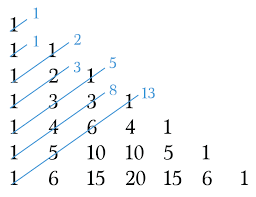
\includegraphics{FibPascal.png}

\end{document}
